\documentclass{article}
\usepackage[utf8]{inputenc}
\usepackage{graphicx}
\usepackage{amsmath}
\usepackage{geometry}
\usepackage{pdfpages}
\usepackage{hyperref}
\usepackage{enumitem}
\usepackage{listings}
\usepackage{setspace} % for \onehalfspacing and \singlespacing macros
\onehalfspacing 

\usepackage [english]{babel}
\usepackage [autostyle, english = american]{csquotes}
\MakeOuterQuote{"}

\usepackage{etoolbox}
\AtBeginEnvironment{quote}{\singlespacing\small}


\newcommand{\link}[1]{{\color{blue}\href{#1}{#1}}}


\geometry{margin=1.5in}
\title{A REGRESSION ANALYSIS OF THE STRATEGIC SUBJECT LIST\thanks{This work was not supported by any organization. Ethan Sargent graduated from Harvey Mudd College in 2019 with a B.S. in Mathematics. Contact: {\tt esargent at hmc dot edu }}}
\author{Ethan Sargent}
\date{\today}

\begin{document}

\maketitle
\newpage
 

\section{Statement of Intent}
The Strategic Subject Algorithm (SSA) was developed at the Illinois Institute of Technology in 2013 and ranked hundreds of thousands of Chicagoans based on their estimated likelihood of involvement in a shooting, as either as a victim or a perpetrator \cite{nyt}.\\\\
After a FOIA request by the Chicago Sun-Times \cite{upturn}, the City of Chicago released the 2017 version of the Strategic Subject List (SSL), which is available at \cite{data}. Each row of the list represents a subject. Fields include each subject's SSL score, the 8 fields used as inputs to the SSA in computing this score, and 44 other fields including such sensitive information as race, gender, and geographical location that the algorithm does not incorporate. The details of the algorithm itself are not public, nor are the criteria for inclusion on the list - per \cite{upturn}, "127,513 individuals on the list have never been arrested or shot." These criteria and the algorithm itself are periodically updated - only 102 of the 398,684 subjects on the most recent list have no recent arrest date.\\\\
The New York Times \cite{nyt} and Upturn \cite{upturn} conducted highly successful regression analyses of SSL score, although they did not publicize the details of their models. What follows is an additional regression analysis which is therefore not intended as original research, but is instead offered in the spirit of exposition on the Strategic Subject Algorithm. We begin with exploratory data analysis of the SSL and its 53 fields. Next, we present several accurate models of SSL score as a function of its 8 predictor variables. Finally, we attend to the obfuscated predictor variable {\tt TREND IN CRIMINAL ACTIVITY}. As with SSL score, the mechanism by which this variable is computed is unknown, so we construct a model which predicts this variable.\\\\
In a Chicago Police Department directive \cite{directive}, the SSL was announced to have been discontinued effective January 9th, 2019. The SSL and SSA were replaced by the Subject Assessment and Information Dashboard (SAID)
 and the Crime and Victimization Risk Model (CVRM), which model is described in detail at \cite{factsheet}. The CVRM takes as inputs 6 of the 8 inputs to the SSA, was also designed by IIT, and appears to have the same function of predicting subjects' short-term likelihood of either committing or being a victim of a shooting. Unlike the SSA, the CVRM represents the subject list as an undirected graph, reflecting IIT's understanding that "[i]n prior research on violent crime, [correlations] have been extensively demonstrated to exist among individuals who are close to one another in a graph defined by co-arrests." To my knowledge no other information about the SAID or the CVRM is available to the public.
%\newline \newline \par ETHAN SARGENT

%Add Picture in and Uncomment
%\par \includegraphics[width=4cm,height=2cm]{Final/1_Writing/sign.png}
%\par \today   

The Strategic Subject Algorithm (SSA) was developed at the Illinois Institute of Technology in 2013 and ranked hundreds of thousands of Chicagoans based on their estimated likelihood of involvement in a shooting, as either as a victim or a perpetrator \cite{nyt}.\\\\
After a FOIA request by the Chicago Sun-Times \cite{upturn}, the City of Chicago released the 2017 version of the Strategic Subject List (SSL), which is available at \cite{data}. Each row of the list represents a subject. Fields include each subject's SSL score, the 8 fields used as inputs to the SSA in computing this score, and 44 other fields including such sensitive information as race, gender, and geographical location that the algorithm does not incorporate. The details of the algorithm itself are not public, nor are the criteria for inclusion on the list - per \cite{upturn}, "127,513 individuals on the list have never been arrested or shot." These criteria and the algorithm itself are periodically updated - only 102 of the 398,684 subjects on the most recent list have no recent arrest date.\\\\
The New York Times \cite{nyt} and Upturn \cite{upturn} conducted highly successful regression analyses of SSL score, although they did not publicize the details of their models. What follows is an additional regression analysis which is therefore not intended as original research, but is instead offered in the spirit of exposition on the Strategic Subject Algorithm. We begin with exploratory data analysis of the SSL and its 53 fields. Next, we present several accurate models of SSL score as a function of its 8 predictor variables. Finally, we attend to the obfuscated predictor variable {\tt TREND IN CRIMINAL ACTIVITY}. As with SSL score, the mechanism by which this variable is computed is unknown, so we construct a model which predicts this variable.\\\\
In a Chicago Police Department directive \cite{directive}, the SSL was announced to have been discontinued effective January 9th, 2019. The SSL and SSA were replaced by the Subject Assessment and Information Dashboard (SAID)
 and the Crime and Victimization Risk Model (CVRM), which model is described in detail at \cite{factsheet}. The CVRM takes as inputs 6 of the 8 inputs to the SSA, was also designed by IIT, and appears to have the same function of predicting subjects' short-term likelihood of either committing or being a victim of a shooting. Unlike the SSA, the CVRM represents the subject list as an undirected graph, reflecting IIT's understanding that "[i]n prior research on violent crime, [correlations] have been extensively demonstrated to exist among individuals who are close to one another in a graph defined by co-arrests." To my knowledge no other information about the SAID or the CVRM is available to the public.
%\newline \newline \par ETHAN SARGENT

%Add Picture in and Uncomment
%\par \includegraphics[width=4cm,height=2cm]{Final/1_Writing/sign.png}
%\par \today   

\newpage

\section{Table of Contents}
\tableofcontents
\newpage

\section{Exploratory Data Analysis}
\subsection{A word on the dataset}
\subsubsection{Missing values}
The Strategic Subject List has 398,684 rows, each of which represents an individual on the list. The list has 53 fields: 8 predictor fields, which the CPD claims are the only fields used in computing the SSL Score, 44 other fields including variables like race, sex, and geographical location, and the SSL Score itself. Among the 8 predictor columns and the SSL Score column, there are 102 rows with missing values. Since the dataset is large, we elect to drop these rows rather than impute or interpolate these missing values.
\subsubsection{Preprocessing}
There are two predictor variables that need to be interpreted before they are useful as inputs to a regression analysis. First, the field \texttt{PREDICTOR RAT AGE AT LATEST ARREST} is given as a string: ‘less than 20’ if the individual was younger than 20 at the time of their most recent arrest, and otherwise as a decade-long range; for instance, ‘20-30’ if the subject was between 20 and 30 at the time of their most recent arrest. These obfuscations are presumably to preserve anonymity. To convert these values to numerical inputs that preserve distance, we convert ‘less than 20’ observations to the value 0.0, ‘20-30’ observations to the value 1.0, ‘30-40’ observations to the value 2.0, and so on.\\\\
Second, the field \texttt{PREDICTOR RAT GANG AFFILIATION} is a binary categorical variable, with ‘1’ indicating an outstanding gang affiliation. We use this as a dummy variable in the regression analysis, treating it like any other continuous input to the model. The coefficient on the dummy variable in a linear regression analysis then becomes a differential intercept coefficient. That is to say, our predictions for gang affiliated individuals differ from our predictions for non-gang affiliated individuals only by a constant value fitted by the model. Per \cite{upturn}, gang affiliation is no longer used as an input to the model and was never a particularly effective predictor, however, the most recent publicly available SSL has scores computed using gang affiliation, so we include it in our model.
\subsection{The distributions of SSL score and its 8 predictor variables}
SSL scores are computed using an algorithm which takes the following eight fields as inputs\\
\begin{enumerate}[nolistsep]
    \item \texttt{PREDICTOR RAT AGE AT LATEST ARREST}
    \item \texttt{PREDICTOR RAT VICTIM SHOOTING INCIDENTS}
    \item \texttt{PREDICTOR RAT VICTIM BATTERY OR ASSAULT}
    \item \texttt{PREDICTOR RAT ARRESTS VIOLENT OFFENSES}
    \item \texttt{PREDICTOR RAT GANG AFFILIATION}
    \item \texttt{PREDICTOR RAT NARCOTIC ARRESTS}
    \item \texttt{PREDICTOR RAT TREND IN CRIMINAL ACTIVITY}
    \item \texttt{PREDICTOR RAT UUW ARRESTS}\\
\end{enumerate}

The distributions of SSL Scores and the above variables are shown below. Predictors 2-4, 6, and 8 are heavily skewed right. Visibility is improved a little by putting them on a log-scale. Normalizing predictor 7 is unhelpful due to the existence of extreme outliers.

\begin{center}
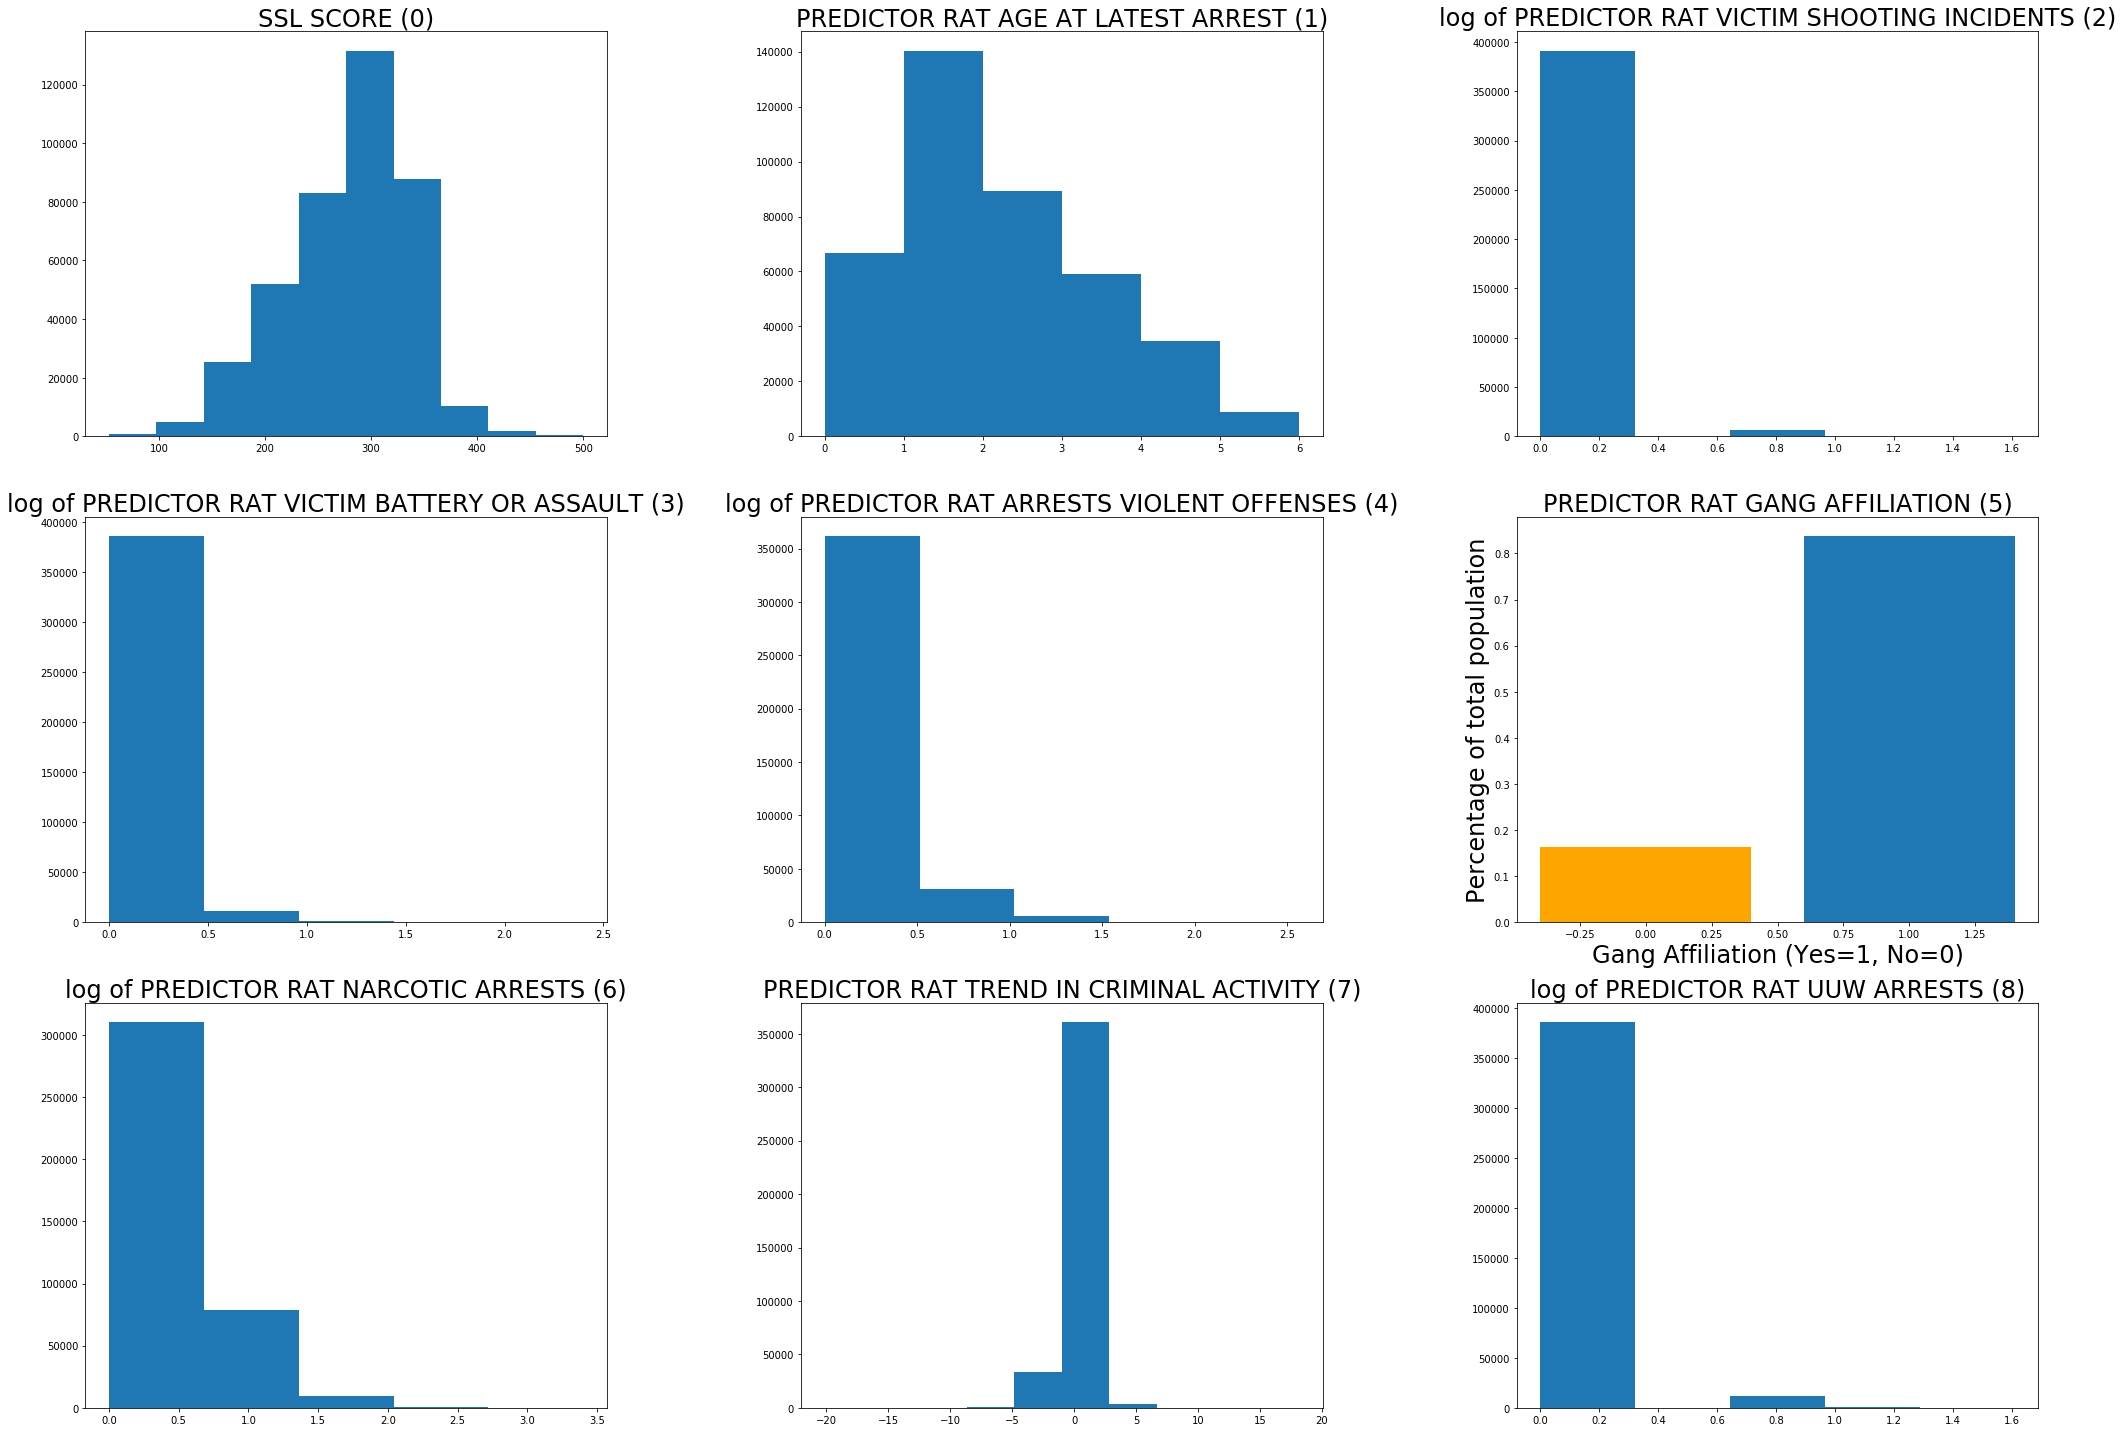
\includegraphics[scale=.2]{images/distribs.png}
\end{center}

\subsubsection{SSL scores: a summary}
SSL Scores have minimum $53$, maximum $500$, mean $279.90$, and standard deviation $57.88$. They fail a normality test. 153 individuals have the maximum score of $500$, while only $132$ have scores between $480$ and $499$, suggesting some degree of bunching at the right tail. 95\% of individuals have an SSL score between $157$ and $372$.

\subsection{Exploring a model of \texttt{PREDICTOR RAT TREND IN CRIMINAL ACTIVITY}}
The way \texttt{PREDICTOR RAT TREND IN CRIMINAL ACTIVITY} (hereafter, \texttt{TREND}) is computed is unknown. A regression analysis of \texttt{TREND} will eventually factor in to our analysis. For now, we examine its distribution and remark on its relationships to other fields in the list.

\subsubsection{The distribution of \texttt{TREND}}
The distribution fails a normality test. $95$\% of the data lies between $-.9$ and $.7$, and $99$\% of the data between $-1.6$ and $1.3$. However, the distribution has many extreme outliers. The maximum and minimum are both approximately twenty standard deviations from the mean, and there are $238$ values 8 or more standard deviations from the mean. A histogram of \texttt{TREND} is a little more revealing with 1000 left and right outliers truncated.
\begin{center}
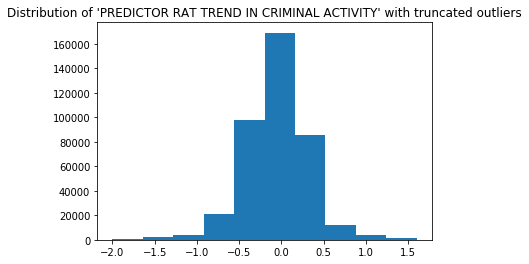
\includegraphics[scale=.8]{images/trends.png}
\end{center}
An upward spike in criminal activity (the highest 100 of observed \texttt{TREND} values) almost always is associated with a \texttt{LATEST DATE} of 2016. The low end \texttt{TREND} has a mean \texttt{LATEST DATE} of $2014.76$. In contrast, the list as a whole has a mean \texttt{LATEST DATE} of $2014.20$. One possible explanation: an active criminal who has not committed a crime recently ought to have a lower trend than someone who has simply not committed a crime recently.\\\\
We use the \texttt{fitter} module to investigate possible distributions. The \texttt{fitter} module compares the observed distribution to \texttt{scipy}'s 80 distributions - for each of \texttt{scipy}'s continuous distributions, the `.fit` function returns a maximum likelihood estimate for the parameters of the distribution given that the observed data is of that distribution. Then, \texttt{fitter} finds the distribution that minimizes the squared-error discrepancy between the observed and predicted data.\\\\
The \texttt{exponnorm} distribution is perhaps the most intuitive of these fits since it has a low squared error and an interpretation as the sum of normal and exponential random variables, which variables are possibly inputs to the calculation of \texttt{TREND}.\\\\
Below we compare the distribution of simulated, fitted \texttt{exponnorm} values to that of observed \texttt{TREND} values. As evidenced by the plots, the \texttt{exponnorm} fails to replicate the heavy tails of the \texttt{TREND} values. While imperceptible in the left histogram, the outliers of \texttt{TREND} skew the bin width much higher than in the histogram of the simulated values. We correct for this in the right histogram - nevertheless, \texttt{exponnorm} is a poor choice of distribution.
\begin{center}
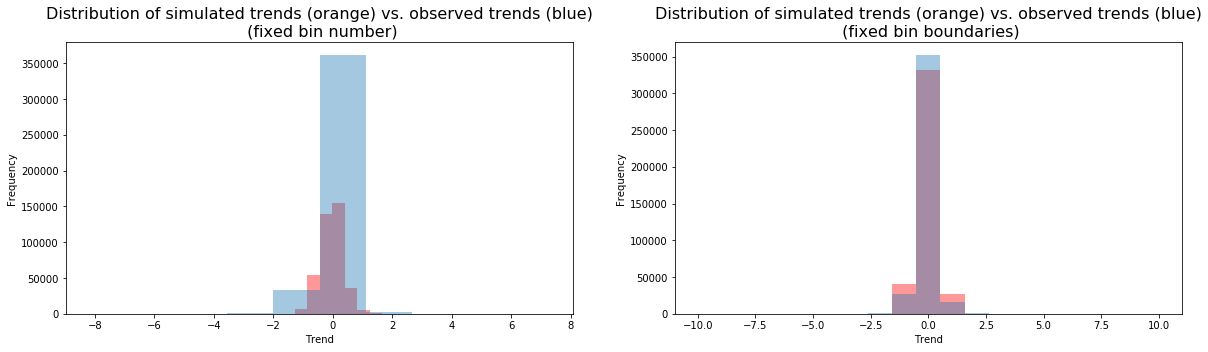
\includegraphics[scale=.3]{images/sim_vs_obs.png}
\end{center}

\subsubsection{Comparing \texttt{TREND} to the SSA's unused fields}
In addition to the seven \texttt{PREDICTOR} fields, our analysis will require interpretation of the remaining 44 fields. We are specifically interested in whether there is evidence that \texttt{PREDICTOR RAT TREND IN CRIMINAL ACTIVITY} is derived from these fields, which the CPD claims are not inputs to the model. In addition to the predictor fields, the following fields warrant investigation:\\
\begin{enumerate}[nolistsep]
    \item \texttt{LATEST DATE}: (latest date of police contact)
    \item \texttt{WEAPONS ARR CNT} (counts are computed from arrests in last 10 years)
    \item \texttt{LATEST WEAPON ARR DATE}
    \item \texttt{NARCOTICS ARR CNT}
    \item \texttt{LATEST NARCOTIC ARR DATE}
    \item \texttt{DOMESTIC ARR CNT}
    \item \texttt{LATEST DOMESTIC ARR DATE}
    \item \texttt{SSL LAST PTV DATE} (from the third footnote: “Most recent date that the subject was matched with a victim or arrest record making the subject a ‘Party to Violence’)\\
\end{enumerate}
Roughly 75.8\% of the entries in these fields are \texttt{NaN}. This makes sense - most people will not have, for instance a \texttt{LATEST DOMESTIC ARR DATE}, since most people have not been arrested for domestic violence. These are therefore not “missing values” in the traditional sense, and so it would be inappropriate to simply drop them from the model. Dropping every row with an \texttt{NaN} value in any of the above fields would leave only individuals with a large, diverse criminal record - this sampling bias would corrupt the resulting analysis. Our representation of these values will ultimately depend on model choice.

\subsubsection{\texttt{LATEST DATE} vs. \texttt{TREND}}
The below box plot indicates that the vast majority of subjects have a \texttt{TREND} near $0$, regards of the year of their \texttt{LATEST DATE} of police contact. There is a slight positive correlation between 'trend' and \texttt{LATEST DATE} of .4712, with a $p$ value of $0$.\\\\
Yet it is possible that not all police contact is bad for one's 'trend'. In the year 2016, for example, many subjects have an incredibly low 'trend' value that coincides with a recent date of police contact. It is unknown what qualifies as police contact: an arrest might warrant an increase in 'trend', whereas an interview leading the CPD to conclude a subject is no longer gang affiliated, for instance, might warrant a decrease in 'trend'. Per \cite{upturn}:
\begin{quote}
The CPD claims the SSL is used in conjunction another program, called Custom Notifications (Special Order S10–05), where police officers, social workers, and community leaders “deliver a joint message ... informing [people on the list] of their risk for prosecution based on criminal history, and explaining their opportunities for community help and support.” The CPD itself describes Custom Notifications as “a process that identifies potential criminal actors and victims associated with the continuum of violence. Once identified, the individual is notified of the consequences that will result should violent activity continue.” Between 2013 and 2016, the CPD is reported to have made over 1,400 of these visits.
\end{quote}
\begin{center}
    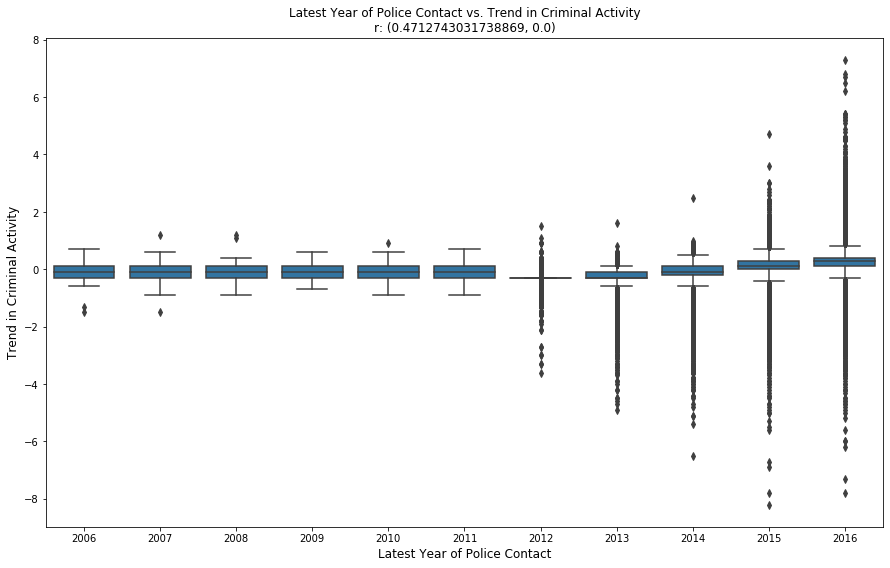
\includegraphics[scale=.4]{images/trend_vs_date.png}
\end{center}
The boxplot for the year 2013 is not an error - roughly 29,000 of the 30,000 subjects for that year have \texttt{TREND} value $-.3$, which encompasses the second and third quartiles. This anomaly in \texttt{TREND} computation will doubtless affect our model.
\subsubsection{Arrest counts and \texttt{TREND}:}
Below are three scatterplots. They depict one of three types of arrest count (weapons, narcotics, domestic) vs. \texttt{TREND}. These plots reveal they are unlikely to be helpful in any model. We note that the distribution of \texttt{WEAPONS ARR CNT} is much tighter than those of \texttt{NARCOTICS ARR CNT} and \texttt{DOMESTIC ARR CNT}. Illinois has relatively strict gun control laws; per a Chicago criminal defense lawyer, possession of a loaded gun with no FOID/CCL card carries a penalty of 1-3 years in prison with steeper penalties for repeat offenders and other aggravating factors.\cite{lawyer} It is likely that subjects don't accumulate many weapons charges due to the high probability of lengthy incarceration that accompanies each arrest.
\begin{center}
    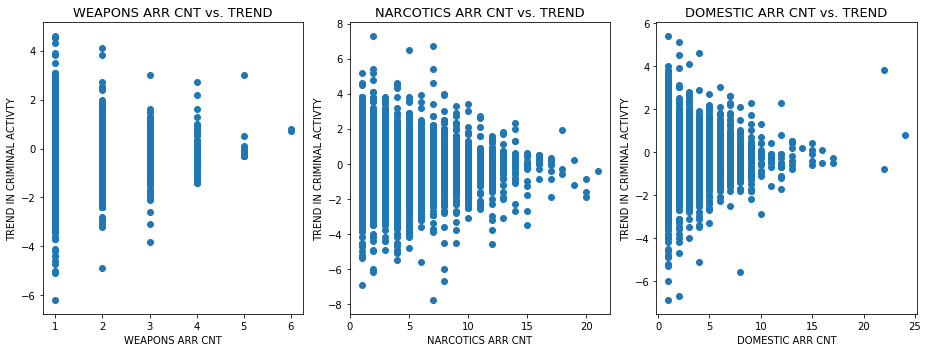
\includegraphics[scale=.4]{images/arrest_counts.png}
\end{center}
\subsubsection{Recent arrest dates and \texttt{TREND}:}
Here we come across more related variables. \texttt{LATEST WEAPON ARR DATE} has the strongest correlation we have seen yet with \texttt{TREND}: $.41$. \texttt{LATEST DOMESTIC ARR DATE} and \texttt{LATEST NARCOTICS ARR DATE} have correlations of $.12$ and $.14$, respectively. In the boxplots below the correlations are visible in the slight positive trends of the means.
\begin{center}
    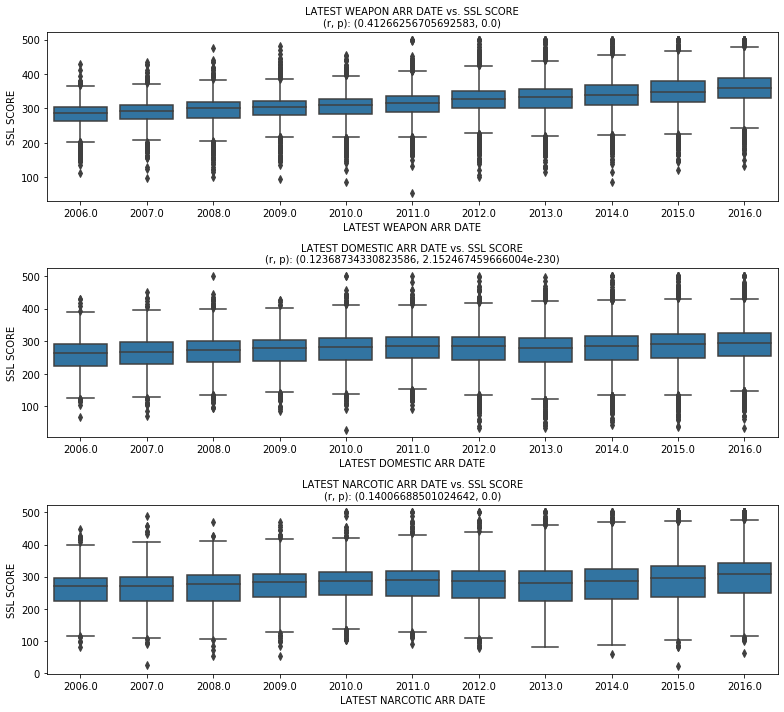
\includegraphics[scale=.4]{images/latest_arrests.png}
\end{center}

\subsection{Age}
Both Upturn and the New York Times found that the variable most closely related to SSL score was age. Concretely, \cite{nyt} found that
\begin{quote}
The most significant characteristic for computing an S.S.L. risk score is the age of a potential victim or offender. For every decade of age, the risk score declined by about 40 points. Practically speaking, this variable limits the list to young people: No one older than 30 falls within the highest-risk category with a score at or above 480.
\end{quote}
And similarly, \cite{upturn} found that
\begin{quote}
    age accounts for roughly 89\% of variance in SSL scores. In other words, the score mostly just reflects each person’s age.
\end{quote}
So, age is a crucial ingredient for modeling SSL score. Below we have a scatter plot of age group vs. SSL score. We replicate Upturn's finding that age accounts for $.9412^2 \sim 89$\% of the variance in SSL scores, although we are unsure whether they used the same age-group-to-continuous-variable conversion. Recall that ours was 'less than 20' $\to 0$, '20-30' $\to 1$, '30-40' $\to 2$ and so on.
\begin{center}
    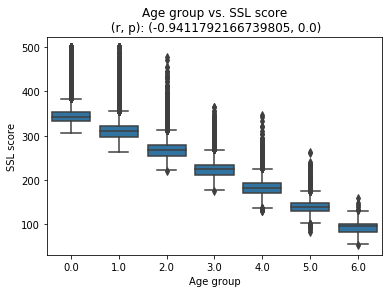
\includegraphics[scale=.7]{images/age_vs_ssl.png}
\end{center}
There are two other fields on the list pertaining to age. \texttt{AGE TO} (per \cite{data}: "If Age is an estimated range, this is the upper end of that range") and  \texttt{AGE GROUP} (per \cite{data}: "Subject's Age as of their latest arrest record"). In any case, these fields contain  which exactly the same values. Since \texttt{AGE CURR} values are higher or equal, we assume these fields were deprecated and will use \texttt{AGE CURR} exclusively.
\subsubsection{The relationship between \texttt{AGE CURR} and \texttt{PREDICTOR RAT AGE AT LATEST ARREST}}
About 77\% of subjects are, as of May 1, 2017 when the data was last updated, the same age as when they were last arrested. Interestingly, 924 subjects are listed to have a current age less than their age at the time of their latest arrest. Since this is impossible, it is possible when a subject is arrested, their current age is not updated. The 2D histogram below indicates that there is a high density of subjects along the line \texttt{AGE CURR} = \texttt{PREDICTOR RAT AGE AT LATEST ARREST}, with over a quarter of subjects ((28.6\%, the yellow square) both between 20 and 30 and with a most recent arrest date while between 20 and 30.
\begin{center}
    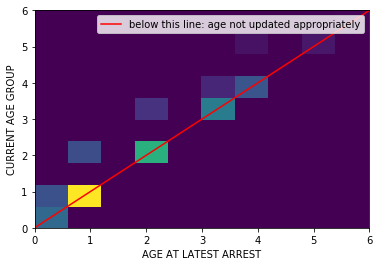
\includegraphics[scale=.5]{images/age_at_latest_arrest.png}
\end{center}

\subsection{Location}
Latitude and longitude data are provided for location of the subject's most recent arrest, but only for 224,235 subjects, or $56.24$\% of the total. The situation is not much improved for census tract and community area fields, which are non-null for just 227,763 and 224,311 rows, respectively. Since 398,582 subjects have a non-null entry for \texttt{PREDICTOR RAT AGE AT LATEST ARREST}, we assume at least 398,582 subjects have been arrested, and therefore these location fields are woefully incomplete.\\\\
Below is a heatmap of of arrests based on the available latitude and longitude data. The one yellow square is adjacent to West and East Garfield Park - per the Chicago Tribune, these are two of the highest-crime neighborhoods in Chicago.\cite{crime}
\begin{center}
    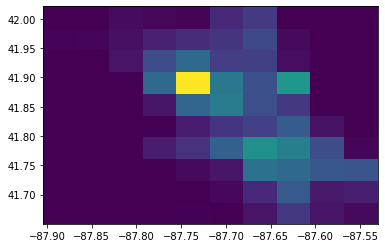
\includegraphics[scale=.5]{images/locations.png}
\end{center}

\subsection{Race and gender}
Per the CPD, the algorithm does not take this sensitive information as input. Some analysis is recorded here for posterity, although it does not suggest vast differences in SSL score across race and sex. Nevertheless, we conduct two $F$-tests below which lead us to reject the null hypotheses that SSL scores do not depend on race or sex. Since SSL scores fail a normality test, we do not observe the normality assumption required for the $F$-test, which luckily is robust to violations of this assumption especially when sample size is large.\\\\
The field \texttt{SEX CODE CD} has value \texttt{M} if the subject is male, \texttt{F} if the subject is female, and \texttt{X} in 57 cases. Presumably in these latter cases either the subject's sex was not recorded or the subject chose not to identify as male or female.\\\\
Per \cite{data}, the field \texttt{RACE CODE CD} uses the encoding "BLK - Black; WHI - White; API - Asian/Pacific Islander; WBH - Black Hispanic; WWH - White Hispanic; I - American Indian/Alaskan Native; U - Unknown." There are 1899 individuals for whom race is unknown. Bar charts of the mean SSL score by race are shown below.
\begin{center}
    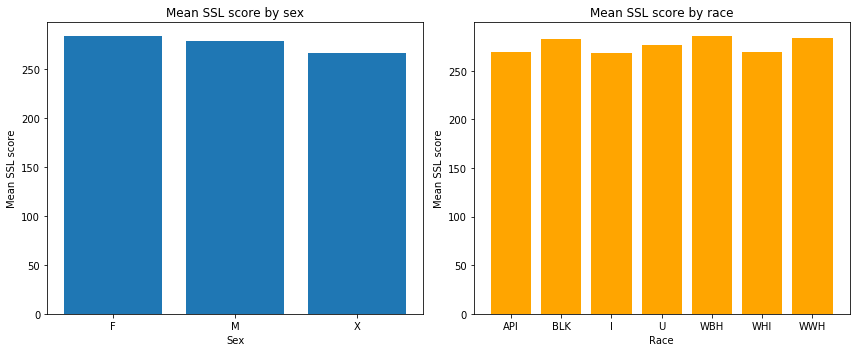
\includegraphics[scale=.5]{images/race.png}
\end{center}
The differences are slight; nevertheless, race and sex have statistically significant impacts on SSL score. One-way F-tests lead us to reject the null hypotheses that SSL score means are the same across these groups. Somewhat surprisingly, females have a higher mean SSL score (283) than males (278). Racial differences in SSL score are more pronounced. Black Hispanics have the highest mean SSL score of 285, whereas Native Americans have the lowest: 268. A table summarizing these results is shown below.
\begin{table}[h!]
\centering
\begin{tabular}{||c c||} 
 \hline
 Race & Mean SSL Score \\ [0.5ex] 
 \hline\hline
\texttt{API}	& $269.433831$\\
\texttt{BLK}	& $282.426208$\\
\texttt{I}	& $268.340580$\\
\texttt{U}	& $276.681938$\\
\texttt{WBH}	& $285.431104$\\
\texttt{WHI} & $269.723842$\\
\texttt{WWH}	& $283.267756$\\ 
 \hline
\end{tabular}
\label{table:1}
\end{table}
\subsection{Gang affiliation}
Gang affiliation is associated with roughly a $10$\% increase in \texttt{SSL SCORE} - unaffiliated subjects (n=333737) have a mean SSL score of 275.170092, whereas gang affiliated subjects (n=64947) have a mean SSL score of 303.835235. After an $F$-test (p = 0.0) we reject the null hypothesis that the difference is statistically insignificant.

\subsection{A word on the dataset}
\subsubsection{Missing values}
The Strategic Subject List has 398,684 rows, each of which represents an individual on the list. The list has 53 fields: 8 predictor fields, which the CPD claims are the only fields used in computing the SSL Score, 44 other fields including variables like race, sex, and geographical location, and the SSL Score itself. Among the 8 predictor columns and the SSL Score column, there are 102 rows with missing values. Since the dataset is large, we elect to drop these rows rather than impute or interpolate these missing values.
\subsubsection{Preprocessing}
There are two predictor variables that need to be interpreted before they are useful as inputs to a regression analysis. First, the field \texttt{PREDICTOR RAT AGE AT LATEST ARREST} is given as a string: ‘less than 20’ if the individual was younger than 20 at the time of their most recent arrest, and otherwise as a decade-long range; for instance, ‘20-30’ if the subject was between 20 and 30 at the time of their most recent arrest. These obfuscations are presumably to preserve anonymity. To convert these values to numerical inputs that preserve distance, we convert ‘less than 20’ observations to the value 0.0, ‘20-30’ observations to the value 1.0, ‘30-40’ observations to the value 2.0, and so on.\\\\
Second, the field \texttt{PREDICTOR RAT GANG AFFILIATION} is a binary categorical variable, with ‘1’ indicating an outstanding gang affiliation. We use this as a dummy variable in the regression analysis, treating it like any other continuous input to the model. The coefficient on the dummy variable in a linear regression analysis then becomes a differential intercept coefficient. That is to say, our predictions for gang affiliated individuals differ from our predictions for non-gang affiliated individuals only by a constant value fitted by the model. Per \cite{upturn}, gang affiliation is no longer used as an input to the model and was never a particularly effective predictor, however, the most recent publicly available SSL has scores computed using gang affiliation, so we include it in our model.
\subsection{The distributions of SSL score and its 8 predictor variables}
SSL scores are computed using an algorithm which takes the following eight fields as inputs\\
\begin{enumerate}[nolistsep]
    \item \texttt{PREDICTOR RAT AGE AT LATEST ARREST}
    \item \texttt{PREDICTOR RAT VICTIM SHOOTING INCIDENTS}
    \item \texttt{PREDICTOR RAT VICTIM BATTERY OR ASSAULT}
    \item \texttt{PREDICTOR RAT ARRESTS VIOLENT OFFENSES}
    \item \texttt{PREDICTOR RAT GANG AFFILIATION}
    \item \texttt{PREDICTOR RAT NARCOTIC ARRESTS}
    \item \texttt{PREDICTOR RAT TREND IN CRIMINAL ACTIVITY}
    \item \texttt{PREDICTOR RAT UUW ARRESTS}\\
\end{enumerate}

The distributions of SSL Scores and the above variables are shown below. Predictors 2-4, 6, and 8 are heavily skewed right. Visibility is improved a little by putting them on a log-scale. Normalizing predictor 7 is unhelpful due to the existence of extreme outliers.

\begin{center}
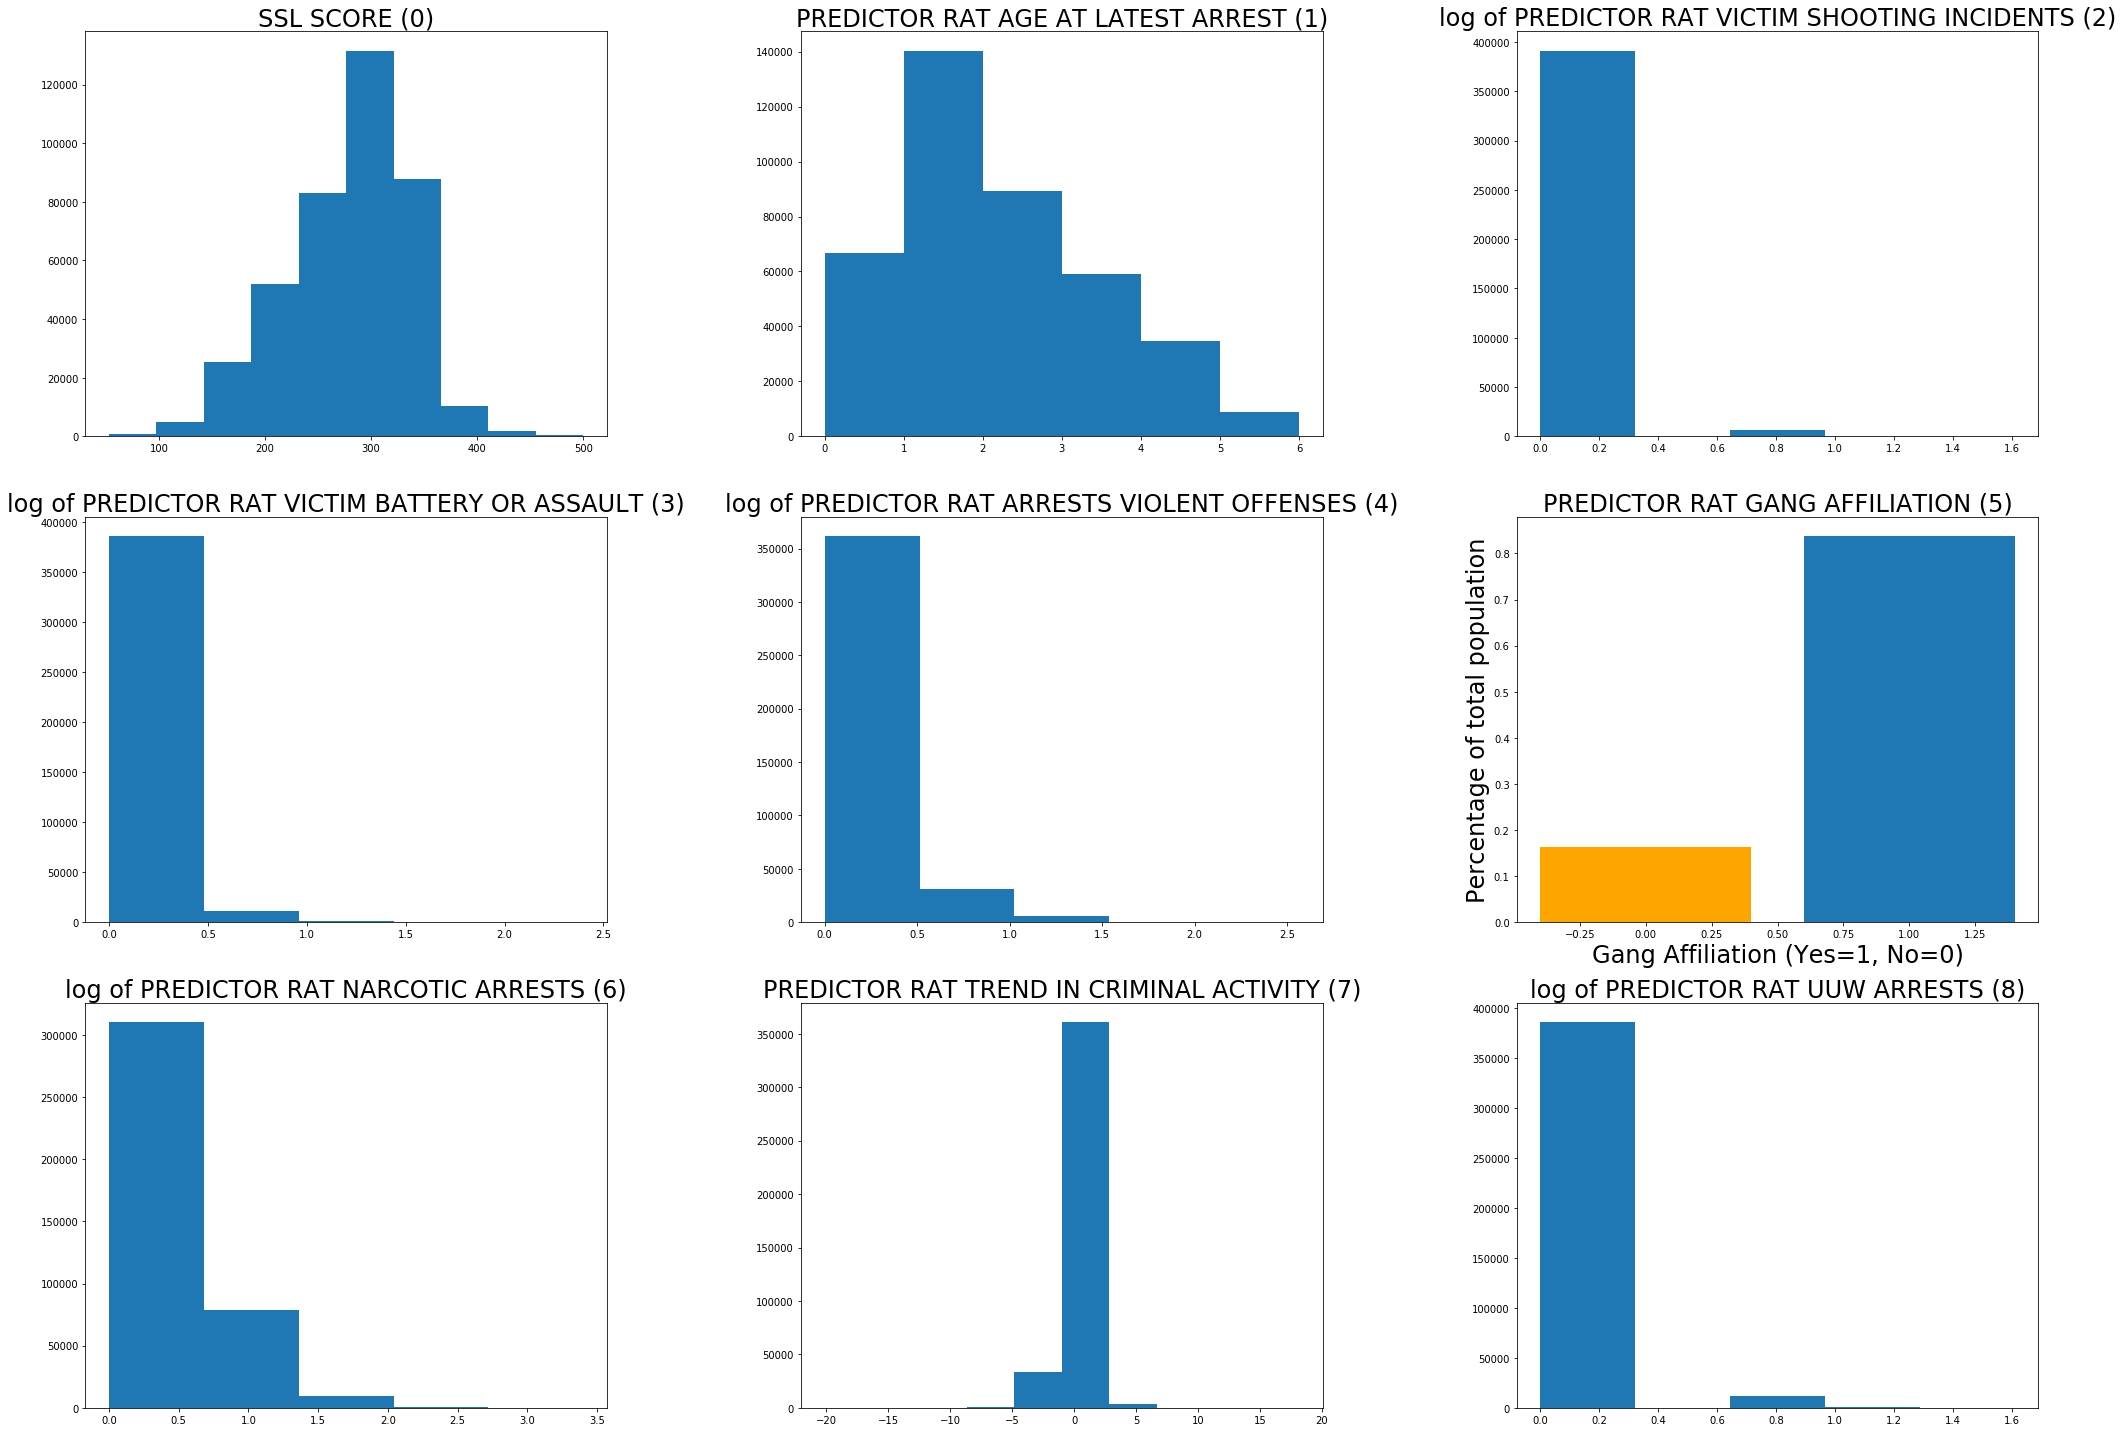
\includegraphics[scale=.2]{images/distribs.png}
\end{center}

\subsubsection{SSL scores: a summary}
SSL Scores have minimum $53$, maximum $500$, mean $279.90$, and standard deviation $57.88$. They fail a normality test. 153 individuals have the maximum score of $500$, while only $132$ have scores between $480$ and $499$, suggesting some degree of bunching at the right tail. 95\% of individuals have an SSL score between $157$ and $372$.

\subsection{Exploring a model of \texttt{PREDICTOR RAT TREND IN CRIMINAL ACTIVITY}}
The way \texttt{PREDICTOR RAT TREND IN CRIMINAL ACTIVITY} (hereafter, \texttt{TREND}) is computed is unknown. A regression analysis of \texttt{TREND} will eventually factor in to our analysis. For now, we examine its distribution and remark on its relationships to other fields in the list.

\subsubsection{The distribution of \texttt{TREND}}
The distribution fails a normality test. $95$\% of the data lies between $-.9$ and $.7$, and $99$\% of the data between $-1.6$ and $1.3$. However, the distribution has many extreme outliers. The maximum and minimum are both approximately twenty standard deviations from the mean, and there are $238$ values 8 or more standard deviations from the mean. A histogram of \texttt{TREND} is a little more revealing with 1000 left and right outliers truncated.
\begin{center}
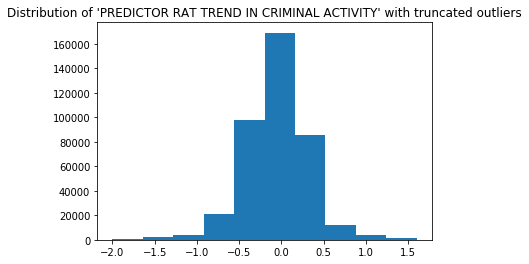
\includegraphics[scale=.8]{images/trends.png}
\end{center}
An upward spike in criminal activity (the highest 100 of observed \texttt{TREND} values) almost always is associated with a \texttt{LATEST DATE} of 2016. The low end \texttt{TREND} has a mean \texttt{LATEST DATE} of $2014.76$. In contrast, the list as a whole has a mean \texttt{LATEST DATE} of $2014.20$. One possible explanation: an active criminal who has not committed a crime recently ought to have a lower trend than someone who has simply not committed a crime recently.\\\\
We use the \texttt{fitter} module to investigate possible distributions. The \texttt{fitter} module compares the observed distribution to \texttt{scipy}'s 80 distributions - for each of \texttt{scipy}'s continuous distributions, the `.fit` function returns a maximum likelihood estimate for the parameters of the distribution given that the observed data is of that distribution. Then, \texttt{fitter} finds the distribution that minimizes the squared-error discrepancy between the observed and predicted data.\\\\
The \texttt{exponnorm} distribution is perhaps the most intuitive of these fits since it has a low squared error and an interpretation as the sum of normal and exponential random variables, which variables are possibly inputs to the calculation of \texttt{TREND}.\\\\
Below we compare the distribution of simulated, fitted \texttt{exponnorm} values to that of observed \texttt{TREND} values. As evidenced by the plots, the \texttt{exponnorm} fails to replicate the heavy tails of the \texttt{TREND} values. While imperceptible in the left histogram, the outliers of \texttt{TREND} skew the bin width much higher than in the histogram of the simulated values. We correct for this in the right histogram - nevertheless, \texttt{exponnorm} is a poor choice of distribution.
\begin{center}
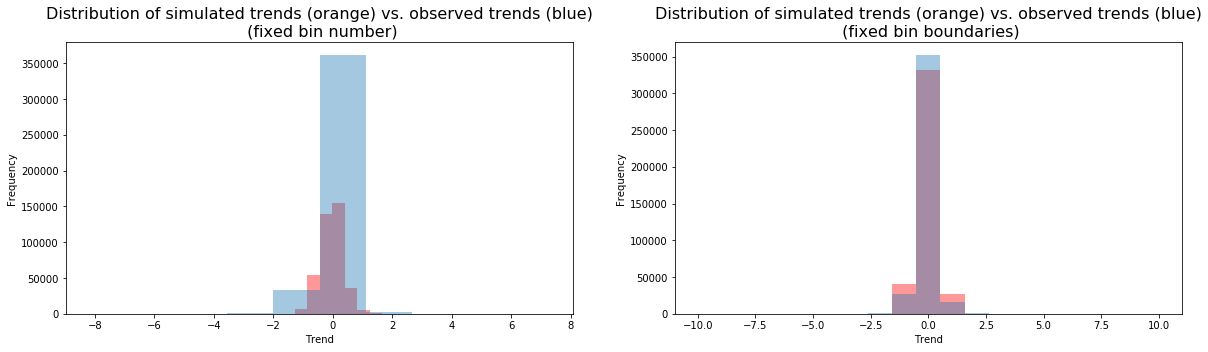
\includegraphics[scale=.3]{images/sim_vs_obs.png}
\end{center}

\subsubsection{Comparing \texttt{TREND} to the SSA's unused fields}
In addition to the seven \texttt{PREDICTOR} fields, our analysis will require interpretation of the remaining 44 fields. We are specifically interested in whether there is evidence that \texttt{PREDICTOR RAT TREND IN CRIMINAL ACTIVITY} is derived from these fields, which the CPD claims are not inputs to the model. In addition to the predictor fields, the following fields warrant investigation:\\
\begin{enumerate}[nolistsep]
    \item \texttt{LATEST DATE}: (latest date of police contact)
    \item \texttt{WEAPONS ARR CNT} (counts are computed from arrests in last 10 years)
    \item \texttt{LATEST WEAPON ARR DATE}
    \item \texttt{NARCOTICS ARR CNT}
    \item \texttt{LATEST NARCOTIC ARR DATE}
    \item \texttt{DOMESTIC ARR CNT}
    \item \texttt{LATEST DOMESTIC ARR DATE}
    \item \texttt{SSL LAST PTV DATE} (from the third footnote: “Most recent date that the subject was matched with a victim or arrest record making the subject a ‘Party to Violence’)\\
\end{enumerate}
Roughly 75.8\% of the entries in these fields are \texttt{NaN}. This makes sense - most people will not have, for instance a \texttt{LATEST DOMESTIC ARR DATE}, since most people have not been arrested for domestic violence. These are therefore not “missing values” in the traditional sense, and so it would be inappropriate to simply drop them from the model. Dropping every row with an \texttt{NaN} value in any of the above fields would leave only individuals with a large, diverse criminal record - this sampling bias would corrupt the resulting analysis. Our representation of these values will ultimately depend on model choice.

\subsubsection{\texttt{LATEST DATE} vs. \texttt{TREND}}
The below box plot indicates that the vast majority of subjects have a \texttt{TREND} near $0$, regards of the year of their \texttt{LATEST DATE} of police contact. There is a slight positive correlation between 'trend' and \texttt{LATEST DATE} of .4712, with a $p$ value of $0$.\\\\
Yet it is possible that not all police contact is bad for one's 'trend'. In the year 2016, for example, many subjects have an incredibly low 'trend' value that coincides with a recent date of police contact. It is unknown what qualifies as police contact: an arrest might warrant an increase in 'trend', whereas an interview leading the CPD to conclude a subject is no longer gang affiliated, for instance, might warrant a decrease in 'trend'. Per \cite{upturn}:
\begin{quote}
The CPD claims the SSL is used in conjunction another program, called Custom Notifications (Special Order S10–05), where police officers, social workers, and community leaders “deliver a joint message ... informing [people on the list] of their risk for prosecution based on criminal history, and explaining their opportunities for community help and support.” The CPD itself describes Custom Notifications as “a process that identifies potential criminal actors and victims associated with the continuum of violence. Once identified, the individual is notified of the consequences that will result should violent activity continue.” Between 2013 and 2016, the CPD is reported to have made over 1,400 of these visits.
\end{quote}
\begin{center}
    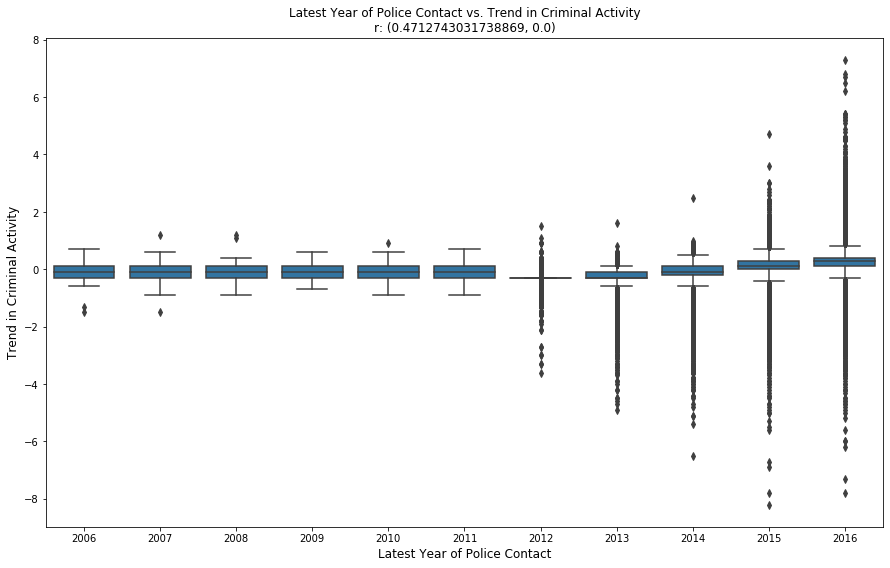
\includegraphics[scale=.4]{images/trend_vs_date.png}
\end{center}
The boxplot for the year 2013 is not an error - roughly 29,000 of the 30,000 subjects for that year have \texttt{TREND} value $-.3$, which encompasses the second and third quartiles. This anomaly in \texttt{TREND} computation will doubtless affect our model.
\subsubsection{Arrest counts and \texttt{TREND}:}
Below are three scatterplots. They depict one of three types of arrest count (weapons, narcotics, domestic) vs. \texttt{TREND}. These plots reveal they are unlikely to be helpful in any model. We note that the distribution of \texttt{WEAPONS ARR CNT} is much tighter than those of \texttt{NARCOTICS ARR CNT} and \texttt{DOMESTIC ARR CNT}. Illinois has relatively strict gun control laws; per a Chicago criminal defense lawyer, possession of a loaded gun with no FOID/CCL card carries a penalty of 1-3 years in prison with steeper penalties for repeat offenders and other aggravating factors.\cite{lawyer} It is likely that subjects don't accumulate many weapons charges due to the high probability of lengthy incarceration that accompanies each arrest.
\begin{center}
    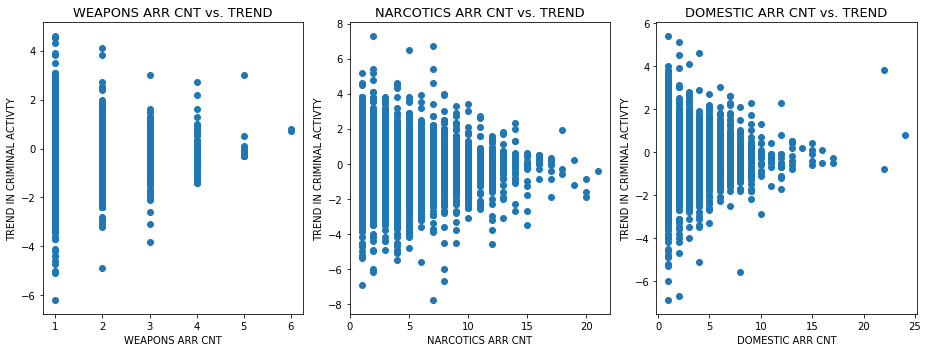
\includegraphics[scale=.4]{images/arrest_counts.png}
\end{center}
\subsubsection{Recent arrest dates and \texttt{TREND}:}
Here we come across more related variables. \texttt{LATEST WEAPON ARR DATE} has the strongest correlation we have seen yet with \texttt{TREND}: $.41$. \texttt{LATEST DOMESTIC ARR DATE} and \texttt{LATEST NARCOTICS ARR DATE} have correlations of $.12$ and $.14$, respectively. In the boxplots below the correlations are visible in the slight positive trends of the means.
\begin{center}
    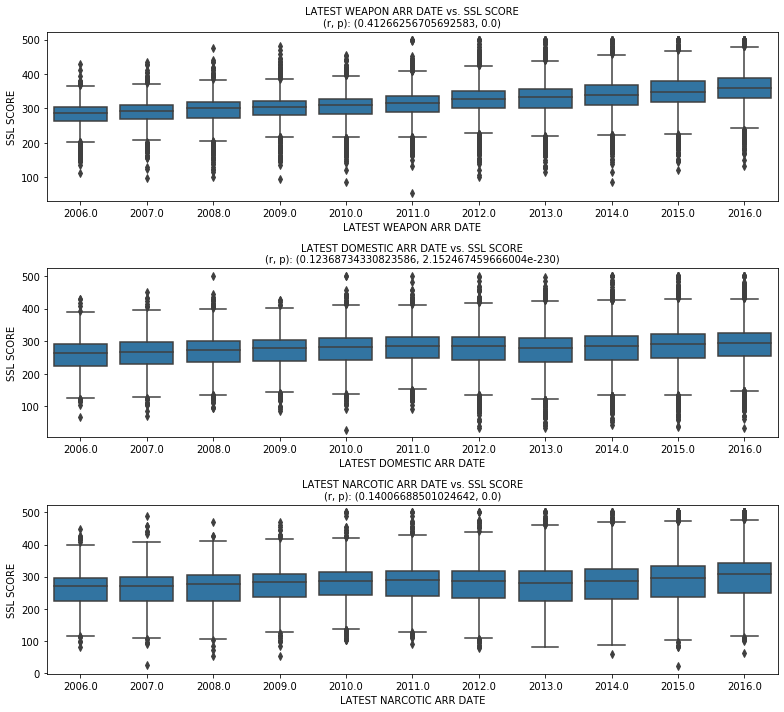
\includegraphics[scale=.4]{images/latest_arrests.png}
\end{center}

\subsection{Age}
Both Upturn and the New York Times found that the variable most closely related to SSL score was age. Concretely, \cite{nyt} found that
\begin{quote}
The most significant characteristic for computing an S.S.L. risk score is the age of a potential victim or offender. For every decade of age, the risk score declined by about 40 points. Practically speaking, this variable limits the list to young people: No one older than 30 falls within the highest-risk category with a score at or above 480.
\end{quote}
And similarly, \cite{upturn} found that
\begin{quote}
    age accounts for roughly 89\% of variance in SSL scores. In other words, the score mostly just reflects each person’s age.
\end{quote}
So, age is a crucial ingredient for modeling SSL score. Below we have a scatter plot of age group vs. SSL score. We replicate Upturn's finding that age accounts for $.9412^2 \sim 89$\% of the variance in SSL scores, although we are unsure whether they used the same age-group-to-continuous-variable conversion. Recall that ours was 'less than 20' $\to 0$, '20-30' $\to 1$, '30-40' $\to 2$ and so on.
\begin{center}
    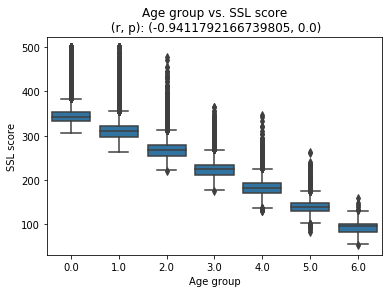
\includegraphics[scale=.7]{images/age_vs_ssl.png}
\end{center}
There are two other fields on the list pertaining to age. \texttt{AGE TO} (per \cite{data}: "If Age is an estimated range, this is the upper end of that range") and  \texttt{AGE GROUP} (per \cite{data}: "Subject's Age as of their latest arrest record"). In any case, these fields contain  which exactly the same values. Since \texttt{AGE CURR} values are higher or equal, we assume these fields were deprecated and will use \texttt{AGE CURR} exclusively.
\subsubsection{The relationship between \texttt{AGE CURR} and \texttt{PREDICTOR RAT AGE AT LATEST ARREST}}
About 77\% of subjects are, as of May 1, 2017 when the data was last updated, the same age as when they were last arrested. Interestingly, 924 subjects are listed to have a current age less than their age at the time of their latest arrest. Since this is impossible, it is possible when a subject is arrested, their current age is not updated. The 2D histogram below indicates that there is a high density of subjects along the line \texttt{AGE CURR} = \texttt{PREDICTOR RAT AGE AT LATEST ARREST}, with over a quarter of subjects ((28.6\%, the yellow square) both between 20 and 30 and with a most recent arrest date while between 20 and 30.
\begin{center}
    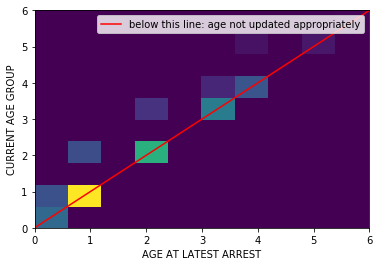
\includegraphics[scale=.5]{images/age_at_latest_arrest.png}
\end{center}

\subsection{Location}
Latitude and longitude data are provided for location of the subject's most recent arrest, but only for 224,235 subjects, or $56.24$\% of the total. The situation is not much improved for census tract and community area fields, which are non-null for just 227,763 and 224,311 rows, respectively. Since 398,582 subjects have a non-null entry for \texttt{PREDICTOR RAT AGE AT LATEST ARREST}, we assume at least 398,582 subjects have been arrested, and therefore these location fields are woefully incomplete.\\\\
Below is a heatmap of of arrests based on the available latitude and longitude data. The one yellow square is adjacent to West and East Garfield Park - per the Chicago Tribune, these are two of the highest-crime neighborhoods in Chicago.\cite{crime}
\begin{center}
    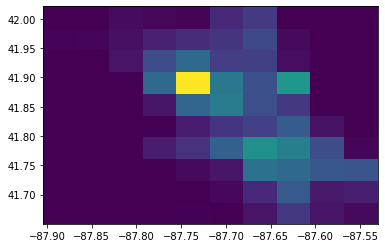
\includegraphics[scale=.5]{images/locations.png}
\end{center}

\subsection{Race and gender}
Per the CPD, the algorithm does not take this sensitive information as input. Some analysis is recorded here for posterity, although it does not suggest vast differences in SSL score across race and sex. Nevertheless, we conduct two $F$-tests below which lead us to reject the null hypotheses that SSL scores do not depend on race or sex. Since SSL scores fail a normality test, we do not observe the normality assumption required for the $F$-test, which luckily is robust to violations of this assumption especially when sample size is large.\\\\
The field \texttt{SEX CODE CD} has value \texttt{M} if the subject is male, \texttt{F} if the subject is female, and \texttt{X} in 57 cases. Presumably in these latter cases either the subject's sex was not recorded or the subject chose not to identify as male or female.\\\\
Per \cite{data}, the field \texttt{RACE CODE CD} uses the encoding "BLK - Black; WHI - White; API - Asian/Pacific Islander; WBH - Black Hispanic; WWH - White Hispanic; I - American Indian/Alaskan Native; U - Unknown." There are 1899 individuals for whom race is unknown. Bar charts of the mean SSL score by race are shown below.
\begin{center}
    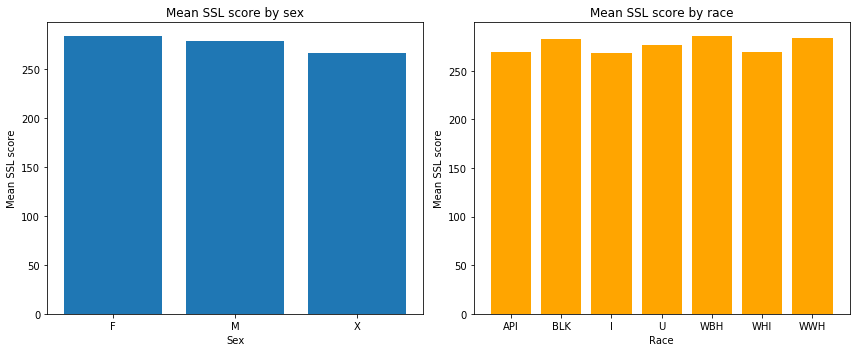
\includegraphics[scale=.5]{images/race.png}
\end{center}
The differences are slight; nevertheless, race and sex have statistically significant impacts on SSL score. One-way F-tests lead us to reject the null hypotheses that SSL score means are the same across these groups. Somewhat surprisingly, females have a higher mean SSL score (283) than males (278). Racial differences in SSL score are more pronounced. Black Hispanics have the highest mean SSL score of 285, whereas Native Americans have the lowest: 268. A table summarizing these results is shown below.
\begin{table}[h!]
\centering
\begin{tabular}{||c c||} 
 \hline
 Race & Mean SSL Score \\ [0.5ex] 
 \hline\hline
\texttt{API}	& $269.433831$\\
\texttt{BLK}	& $282.426208$\\
\texttt{I}	& $268.340580$\\
\texttt{U}	& $276.681938$\\
\texttt{WBH}	& $285.431104$\\
\texttt{WHI} & $269.723842$\\
\texttt{WWH}	& $283.267756$\\ 
 \hline
\end{tabular}
\label{table:1}
\end{table}
\subsection{Gang affiliation}
Gang affiliation is associated with roughly a $10$\% increase in \texttt{SSL SCORE} - unaffiliated subjects (n=333737) have a mean SSL score of 275.170092, whereas gang affiliated subjects (n=64947) have a mean SSL score of 303.835235. After an $F$-test (p = 0.0) we reject the null hypothesis that the difference is statistically insignificant.

\newpage

\section{Modeling SSL score}
%Add PDF in and Uncomment
%\includepdf[width=16cm]{Final/1_Writing/CV.pdf}
Except for ordinary least squares (OLS), data was randomly divided into training (80\% of data) and test (20\% of data) sets, and final performance was measured as root-mean-squared error on the test set. A summary of various modeling efforts is below.
\subsection{Summary}
As far as we know, \cite{nyt} and \cite{upturn} only employed linear regression in their analyses of SSL score,  and with good reason: even ordinary least squares is quite effective at predicting SSL score, and more complicated models do not significantly outperform linear regression. So we devote most of our analysis to the results of the linear model, which results are most easily interpreted in context.
\begin{table}[h!]
\centering
\begin{tabular}{||c c c||}
 \hline
 Model & RMSE & Cross-validated (\texttt{nfolds}$=5$)\\ [0.5ex] 
 \hline\hline
\texttt{OLS} (age only) & $19.55$ & No\\
\texttt{OLS} & $12.97$ & No\\
\texttt{OLS} w/ polynomial features (deg $\leq 3$) & $12.48$ & No\\
\texttt{Random Forests} & 12.47 & Yes\\
\texttt{XGBoost} & 12.38 & No\\
 \hline
\end{tabular}
\label{table:2}
\end{table}
\subsection{Predictor Multicollinearity} 
A principal component analysis reveals high multicollinearity among the predictors. Furthermore, the first principal component is essentially age, and the second principal component is essentially narcotic arrests. It seems that the true dimensionality of the data is much lower than 8.\\
\centerline{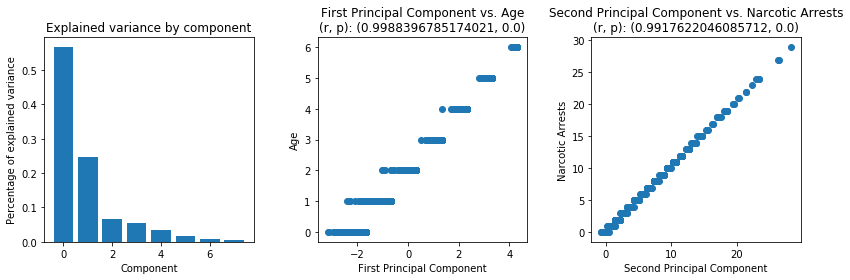
\includegraphics[scale=.55]{images/pca.png}}
In the public description of the CVRM, we find the remark that "inclusion of narcotics arrests and gang affiliation [has] only marginal impact on the results beyond what the model discerns from the other risk factors; therefore, in the current CVRM version, these two risk factors have been omitted."\cite{factsheet} If age and narcotic arrests capture most of the variance in the predictors as indicated by the figure above, the omission of narcotic arrests in the CVRM may reflect an understanding that narcotic arrests is approximately a weighted combination of other inputs.
\subsection{Predictor Strengths}
Recall \cite{upturn} found that age accounts for $89$\% of the variance in SSL score - unsurprisingly, age at latest arrest is by far the most important predictor across all our models. We can assess the relative importance of the predictors for our models concretely: a multiple linear regression on standardized predictors yields coefficients that are just the relative strengths of the predictors. Furthermore, we can assess a predictor's importance to a random forests regression by its total variance reduction across all nodes that split on that feature. Concretely, we have the below barplots.
\begin{center}
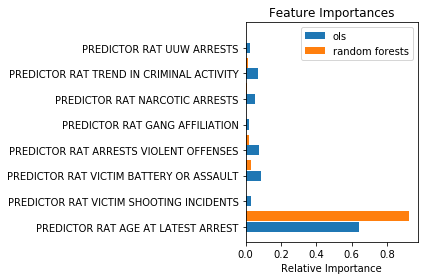
\includegraphics[scale=.7]{images/feature_importances.png}
\end{center}
In the linear model, age is the strongest predictor ($63.91$\% relative importance), while being a victim of a battery or assault is the second strongest predictor ($7.07$\%), followed by arrests for violent offenses ($6.04$\%) and trend in criminal activity ($5.75$\%). In a random forests regression, age is even more dominant at $92.67$\% relative importance - the next highest predictor, being a victim of a battery or assault, only has $2.80$\% relative importance.
\\\\
\newpage
%Add PDF in and Uncomment
%\includepdf[width=16cm]{Final/1_Writing/CV.pdf}
Except for ordinary least squares (OLS), data was randomly divided into training (80\% of data) and test (20\% of data) sets, and final performance was measured as root-mean-squared error on the test set. A summary of various modeling efforts is below.
\subsection{Summary}
As far as we know, \cite{nyt} and \cite{upturn} only employed linear regression in their analyses of SSL score,  and with good reason: even ordinary least squares is quite effective at predicting SSL score, and more complicated models do not significantly outperform linear regression. So we devote most of our analysis to the results of the linear model, which results are most easily interpreted in context.
\begin{table}[h!]
\centering
\begin{tabular}{||c c c||}
 \hline
 Model & RMSE & Cross-validated (\texttt{nfolds}$=5$)\\ [0.5ex] 
 \hline\hline
\texttt{OLS} (age only) & $19.55$ & No\\
\texttt{OLS} & $12.97$ & No\\
\texttt{OLS} w/ polynomial features (deg $\leq 3$) & $12.48$ & No\\
\texttt{Random Forests} & 12.47 & Yes\\
\texttt{XGBoost} & 12.38 & No\\
 \hline
\end{tabular}
\label{table:2}
\end{table}
\subsection{Predictor Multicollinearity} 
A principal component analysis reveals high multicollinearity among the predictors. Furthermore, the first principal component is essentially age, and the second principal component is essentially narcotic arrests. It seems that the true dimensionality of the data is much lower than 8.\\
\centerline{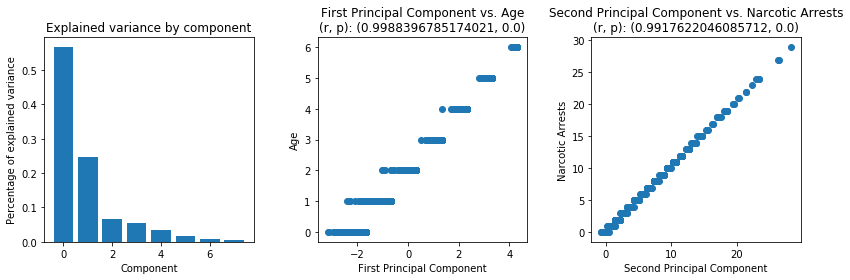
\includegraphics[scale=.55]{images/pca.png}}
In the public description of the CVRM, we find the remark that "inclusion of narcotics arrests and gang affiliation [has] only marginal impact on the results beyond what the model discerns from the other risk factors; therefore, in the current CVRM version, these two risk factors have been omitted."\cite{factsheet} If age and narcotic arrests capture most of the variance in the predictors as indicated by the figure above, the omission of narcotic arrests in the CVRM may reflect an understanding that narcotic arrests is approximately a weighted combination of other inputs.
\subsection{Predictor Strengths}
Recall \cite{upturn} found that age accounts for $89$\% of the variance in SSL score - unsurprisingly, age at latest arrest is by far the most important predictor across all our models. We can assess the relative importance of the predictors for our models concretely: a multiple linear regression on standardized predictors yields coefficients that are just the relative strengths of the predictors. Furthermore, we can assess a predictor's importance to a random forests regression by its total variance reduction across all nodes that split on that feature. Concretely, we have the below barplots.
\begin{center}
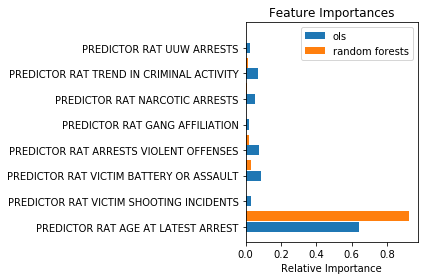
\includegraphics[scale=.7]{images/feature_importances.png}
\end{center}
In the linear model, age is the strongest predictor ($63.91$\% relative importance), while being a victim of a battery or assault is the second strongest predictor ($7.07$\%), followed by arrests for violent offenses ($6.04$\%) and trend in criminal activity ($5.75$\%). In a random forests regression, age is even more dominant at $92.67$\% relative importance - the next highest predictor, being a victim of a battery or assault, only has $2.80$\% relative importance.
\\\\
\newpage
\newpage


\section{Modeling Trend}
%Add PDF in and Uncomment
%\includepdf[pages=1]{Final/1_Writing/Draft_3.pdf}
%\includepdf[pages=2]{Final/1_Writing/Draft_3.pdf}
%\includepdf[pages=3]{Final/1_Writing/Draft_3.pdf}
Overall, our model of \texttt{TREND} was less successful. There is good reason to believe this is due to lack of data. In \cite{factsheet}, which describes the CVRM, an algorithm which has replaced the SSA but takes many of the same inputs including \texttt{TREND}, the authors write that "the 'trend' variable is the slope of a line obtained by a least-squares fit to the individual’s numbers of arrests each year for the past four years." If the trend variable is computed in the same way for the SSL, then the necessary data to compute it is absent from the SSL; in particular, the SSL only contains the year of a subject's most recent arrest, by arrest type, and their arrest count, by arrest type.\\\\
Our pessimism assumes that the trend variables are computed in the same way for the SSL, which may not be the case - if trend is computed strictly from arrests as with the CVRM, it is difficult to see why, for instance, according to the SSL, a man over 60 with no arrests on record has a \texttt{TREND} of $1.2$, which puts him in the $99$th percentile for that variable. Yet we saw in (3.4) that the SSL has non-predictor fields that are internally inconsistent for specific subjects - it is certainly possible that arrest data is not updated properly in the non-predictive fields.\\\\
In sum, the evidence of missing data and the unreliability of the non-predictive entries of the SSL mean that we do not devote as much time and analysis to a model of \texttt{TREND}.
\subsection{Preprocessing}
Recall that our model of \texttt{trend} used 8 fields in addition to the 8 predictor fields of SSL score, and that $75.8$\% of the entries in these additional fields were \texttt{NaN}.\\\\
If an arrest count field, for instance \texttt{NARCOTIC ARR CNT}, is $\texttt{NaN}$, we assume that the subject has does not have a narcotics arrest on record, and we substitute $0$. However, interpreting a time-sensitive fields like \texttt{LATEST DATE} of police contact requires more subtlety. We employed two different strategies for representing these fields as inputs to regression models.
\subsubsection{$0$ substitution}
 We want to preserve distance between values like $2015$ and $2016$, while also ensuring that a subject's \texttt{TREND} is not affected if they have no \texttt{LATEST DATE} - a subject with no police contact is not becoming more or less criminally active over time. Substituting $0$ for \texttt{NaN} values satisfies the second criterion but not the first -  a linear regression fitted to points $0$ and $2015$ will not be able to adequately distinguish between $2015$ and $2016$. This substitution may be adequate for a nonlinear model like random forests or \texttt{xgboost}.
\subsubsection{Slope substitution}
In the spirit of the definition of \texttt{TREND} in \cite{factsheet}, we re-express a subject's most recent arrest date as the slope of the best fit line through the one-hot encoding for that year, where the encoding spans the years 2012-2016, the four years considered by the model described in \cite{factsheet}. For example, if a subject was arrested in 2015, we substitute the slope of the best-fit line through
\[
x=\{2012,2013,2014,2015,2016\}, y=\{0,0,0,1,0\}.
\]
For subjects with a \texttt{LATEST DATE} earlier than 2012 (n=5556), say, $y$, we compute the best-fit slope through
\[
x=\{y, y+1, \hdots, 2011, \hdots, 2016\}, y=\{1,0, \hdots, 0\}.
\]
This substitution has many desirable properties - first, the contribution to \texttt{TREND} of a subject without a recent arrest year is $0$, that is, the slope of the best fit line through the zero vector. Second, recent arrest years have positive slopes which are higher the more recent the year of arrest. Finally, slope tends toward $0$ as  arrest year decreases. A subject's total $\texttt{TREND}$ will be a weighted combination of the subject's slope for each time-sensitive input - \texttt{LATEST DATE}, \texttt{LATEST NARCOTIC ARR DATE}, \texttt{LATEST DOMESTIC ARR DATE}, \texttt{LATEST WEAPON ARR DATE}, and \texttt{SSL LAST PTV DATE} - together with the other inputs.
\subsection{Summary}
Below is a summary of various models of \texttt{TREND}. The random model computes the root-mean-squared error of the difference between the \texttt{TREND} labels and a bootstrap replicate of the \texttt{TREND} labels. A cross-validated random forests regression without a slope substitution is the best performing model.
\\\\
\begin{table}[h!]
\centering
\begin{tabular}{||c c c c||}
 \hline
 Model & Substitution & RMSE & Cross-validated (\texttt{nfolds}$=5$)\\ [0.5ex] 
 \hline\hline
Random model & n/a & $0.5726$ & No\\
\texttt{OLS} & 0 & $0.32786$ & No\\
\texttt{OLS} & slope & $0.3135$ & No\\
\texttt{OLS} w/ polynomial features & 0 & $0.2895$ & No\\
\texttt{OLS} w/ polynomial features & slope & $0.2843$ & No\\
Random forests & 0 & $0.2832$ & Yes\\
Random forests & slope & $0.2848$ & Yes\\
 \hline
\end{tabular}
\label{table:2}
\end{table}

%Add PDF in and Uncomment
%\includepdf[pages=1]{Final/1_Writing/Draft_3.pdf}
%\includepdf[pages=2]{Final/1_Writing/Draft_3.pdf}
%\includepdf[pages=3]{Final/1_Writing/Draft_3.pdf}
Overall, our model of \texttt{TREND} was less successful. There is good reason to believe this is due to lack of data. In \cite{factsheet}, which describes the CVRM, an algorithm which has replaced the SSA but takes many of the same inputs including \texttt{TREND}, the authors write that "the 'trend' variable is the slope of a line obtained by a least-squares fit to the individual’s numbers of arrests each year for the past four years." If the trend variable is computed in the same way for the SSL, then the necessary data to compute it is absent from the SSL; in particular, the SSL only contains the year of a subject's most recent arrest, by arrest type, and their arrest count, by arrest type.\\\\
Our pessimism assumes that the trend variables are computed in the same way for the SSL, which may not be the case - if trend is computed strictly from arrests as with the CVRM, it is difficult to see why, for instance, according to the SSL, a man over 60 with no arrests on record has a \texttt{TREND} of $1.2$, which puts him in the $99$th percentile for that variable. Yet we saw in (3.4) that the SSL has non-predictor fields that are internally inconsistent for specific subjects - it is certainly possible that arrest data is not updated properly in the non-predictive fields.\\\\
In sum, the evidence of missing data and the unreliability of the non-predictive entries of the SSL mean that we do not devote as much time and analysis to a model of \texttt{TREND}.
\subsection{Preprocessing}
Recall that our model of \texttt{trend} used 8 fields in addition to the 8 predictor fields of SSL score, and that $75.8$\% of the entries in these additional fields were \texttt{NaN}.\\\\
If an arrest count field, for instance \texttt{NARCOTIC ARR CNT}, is $\texttt{NaN}$, we assume that the subject has does not have a narcotics arrest on record, and we substitute $0$. However, interpreting a time-sensitive fields like \texttt{LATEST DATE} of police contact requires more subtlety. We employed two different strategies for representing these fields as inputs to regression models.
\subsubsection{$0$ substitution}
 We want to preserve distance between values like $2015$ and $2016$, while also ensuring that a subject's \texttt{TREND} is not affected if they have no \texttt{LATEST DATE} - a subject with no police contact is not becoming more or less criminally active over time. Substituting $0$ for \texttt{NaN} values satisfies the second criterion but not the first -  a linear regression fitted to points $0$ and $2015$ will not be able to adequately distinguish between $2015$ and $2016$. This substitution may be adequate for a nonlinear model like random forests or \texttt{xgboost}.
\subsubsection{Slope substitution}
In the spirit of the definition of \texttt{TREND} in \cite{factsheet}, we re-express a subject's most recent arrest date as the slope of the best fit line through the one-hot encoding for that year, where the encoding spans the years 2012-2016, the four years considered by the model described in \cite{factsheet}. For example, if a subject was arrested in 2015, we substitute the slope of the best-fit line through
\[
x=\{2012,2013,2014,2015,2016\}, y=\{0,0,0,1,0\}.
\]
For subjects with a \texttt{LATEST DATE} earlier than 2012 (n=5556), say, $y$, we compute the best-fit slope through
\[
x=\{y, y+1, \hdots, 2011, \hdots, 2016\}, y=\{1,0, \hdots, 0\}.
\]
This substitution has many desirable properties - first, the contribution to \texttt{TREND} of a subject without a recent arrest year is $0$, that is, the slope of the best fit line through the zero vector. Second, recent arrest years have positive slopes which are higher the more recent the year of arrest. Finally, slope tends toward $0$ as  arrest year decreases. A subject's total $\texttt{TREND}$ will be a weighted combination of the subject's slope for each time-sensitive input - \texttt{LATEST DATE}, \texttt{LATEST NARCOTIC ARR DATE}, \texttt{LATEST DOMESTIC ARR DATE}, \texttt{LATEST WEAPON ARR DATE}, and \texttt{SSL LAST PTV DATE} - together with the other inputs.
\subsection{Summary}
Below is a summary of various models of \texttt{TREND}. The random model computes the root-mean-squared error of the difference between the \texttt{TREND} labels and a bootstrap replicate of the \texttt{TREND} labels. A cross-validated random forests regression without a slope substitution is the best performing model.
\\\\
\begin{table}[h!]
\centering
\begin{tabular}{||c c c c||}
 \hline
 Model & Substitution & RMSE & Cross-validated (\texttt{nfolds}$=5$)\\ [0.5ex] 
 \hline\hline
Random model & n/a & $0.5726$ & No\\
\texttt{OLS} & 0 & $0.32786$ & No\\
\texttt{OLS} & slope & $0.3135$ & No\\
\texttt{OLS} w/ polynomial features & 0 & $0.2895$ & No\\
\texttt{OLS} w/ polynomial features & slope & $0.2843$ & No\\
Random forests & 0 & $0.2832$ & Yes\\
Random forests & slope & $0.2848$ & Yes\\
 \hline
\end{tabular}
\label{table:2}
\end{table}

\newpage

\begin{thebibliography}{9}
\bibitem{nyt} 
J. Asher and R. Arthur, "Inside the Algorithm That Tries to Predict Gun Violence in Chicago."
New York Times, 13 June 2017;
\link{https://www.nytimes.com/2017/06/13/upshot/what-an-algorithm-reveals-about-life-on-chicagos-high-risk-list.html}

\bibitem{upturn} 
B. Posadas, "How strategic is Chicago’s 'Strategic Subjects List'? Upturn investigates."
Medium, 22 June 2017;
\link{https://medium.com/equal-future/how-strategic-is-chicagos-strategic-subjects-list-upturn-investigates-9e5b4b235a7c}

\bibitem{data} 
Chicago Data Portal, 7 December 2017;
\link{https://data.cityofchicago.org/Public-Safety/Strategic-Subject-List/4aki-r3np}

\bibitem{factsheet}
"Crime and Victimization Risk Model (CVRM)." Illinois Insitute of Technology, n.d.;
\link{https://home.chicagopolice.org/wp-content/uploads/2019/01/FACT-SHEET-Crime-and-Victimization-Risk-Model-1.pdf}

\bibitem{directive} 
"SUBJECT ASSESSMENT AND INFORMATION DASHBOARD (SAID)." Chicago Police Department, 09 January 2019.
\link{http://directives.chicagopolice.org/directives/data/a7a57b85-155e9f4b-50c15-5e9f-7742e3ac8b0ab2d3.html?hl=true}

\bibitem{crime} 
"Crime in Chicago: Explore your community." Chicago Tribune, 01 April 2019.
\link{https://www.chicagotribune.com/news/ct-crime-in-chicago-20171114-storygallery.html}

\bibitem{lawyer}
"Gun Charge in Illinois FAQs." Robert J. Callahan: Chicago Criminal Defense Attorney, n.d.; \link{https://www.defenselawyersite.com/gun-charge-in-illinois-faqs/}

\bibitem{sun-times}
M. Dumke and F. Main, "A look inside the watch list Chicago police fought to keep secret." Chicago Sun Times, 18 May 2017.
\link{https://chicago.suntimes.com/2017/5/18/18386116/a-look-inside-the-watch-list-chicago-police-fought-to-keep-secret}

\end{thebibliography}


\end{document}

